\documentclass[a4paper,12pt]{article}

\usepackage{rotating}
\usepackage[top=1in, bottom=1in, left=1in, right=1in]{geometry}
\usepackage{graphicx}
\usepackage[numbers,square,sort&compress]{natbib}
\usepackage{setspace}
\usepackage[cdot,mediumqspace,]{SIunits}
\usepackage{caption}
\usepackage{subcaption}

\begin{document}
\onehalfspacing
\title{Final report of a CTA399 student's work with VLBI pulsar observations}
\author{Natalie Price-Jones}
\date{30 August, 2013}
\maketitle

%%%%%%%%%%%%%%
\begin{abstract}
\label{abstract}

\end{abstract}

%%%%%%%%%%%%%%
\section{Introduction}
\label{sec:introduction}

\subsection{Examples}
\label{sec:ex}

\citep{millisecondpulsar}
\emph{prawn}
(see Figure~\ref{fig:failedFS})
mentioned in section~\ref{sec:git}

\begin{figure}
\centering
\begin{subfigure}{0.5\textwidth}
  \centering
  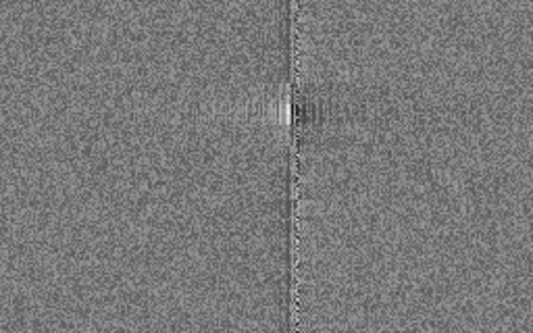
\includegraphics[width=\linewidth]{256ChanLag.pdf}
  \caption{A successful fringestop of Dutta's data using 128 frequency channels. The bright spot is the pulsar.}
  \label{fig:sub1}
\end{subfigure}%
\begin{subfigure}{0.5\textwidth}
  \centering
  
\includegraphics[width=0.8\linewidth]{4096ChanFailedLag.pdf}
  \caption{An example of a possible unsuccessful fringestop lag using 2048 frequency channels. The data is garbled and the pulsar is not visible.}
  \label{fig:sub2}
\end{subfigure}
\caption{Unsuccessful or undesired fringestopping results on the sixth scan taken on pulsar B0329+54 on August 22 2012 by Prasun Dutta.}
\label{fig:failedFS}
\end{figure}

\begin{figure}
\centering

\includegraphics[width=\linewidth]{4096ChanLag.pdf}

\includegraphics[width=\linewidth]{lag102.pdf}
\caption{The results of a successful fringestop using 2048 frequency channels on the same scan used in Figure~\ref{fig:failedFS}. The top image is a cropped section of the bottom one, zoomed to show the pulsar. In the original image, the pulsar is just visible as a white dot in the center. This original image is the exact product of the process used to generate Figure~\ref{fig:sub1} and has a far higher resolution of the pulsar image.}
\label{fig:successfulFS}
\end{figure}


begin{figure}
\centering
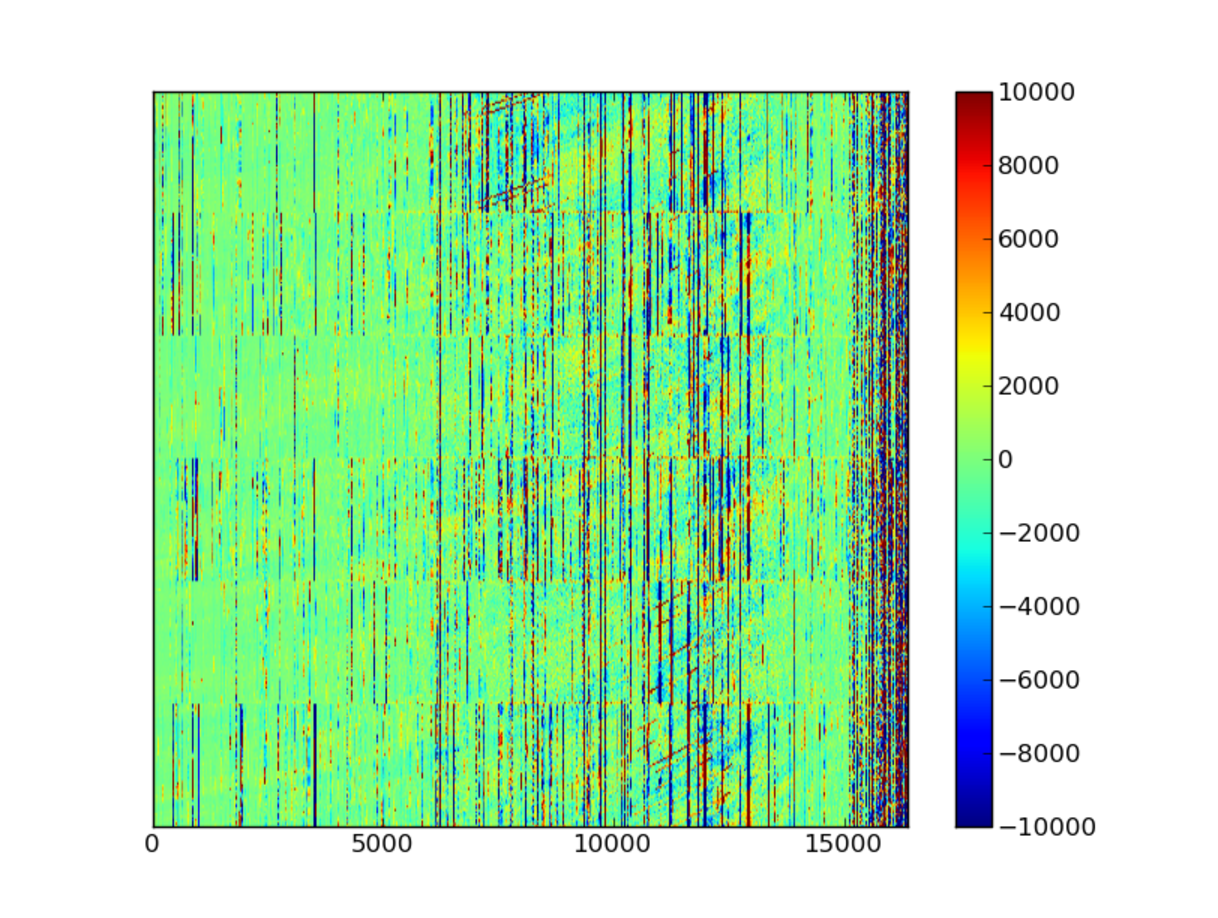
\includegraphics[width=\linewidth]{1919fig1node9.pdf}
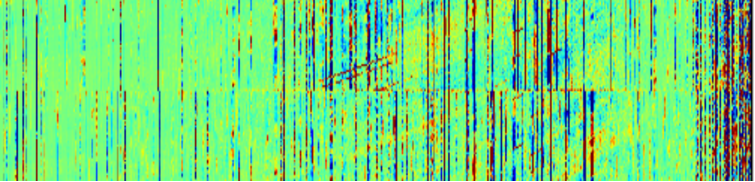
\includegraphics[width=\linewidth]{1919fig1node9crop.pdf}
\caption{A plot of the signal of pulsar B1919+21 folded over 16 minutes with 16384 frequency channels and divided into 6 time bins along the y-axis. The x-axis is the number of the frequency bin, the colourbar the intensity of the signal. The plot shows the polarization recorded to node9. The pulsar is visible as a horizontal line. In this plot, it falls along the division between bins. The cropped portion below is a selection from the first two bins, the pulsar signal following the divide between them. Data was taken July 25 2013.}
\label{fig:folding1919}
\end{figure}

\begin{figure}
\centering
\begin{subfigure}{0.5\textwidth}
  \centering
  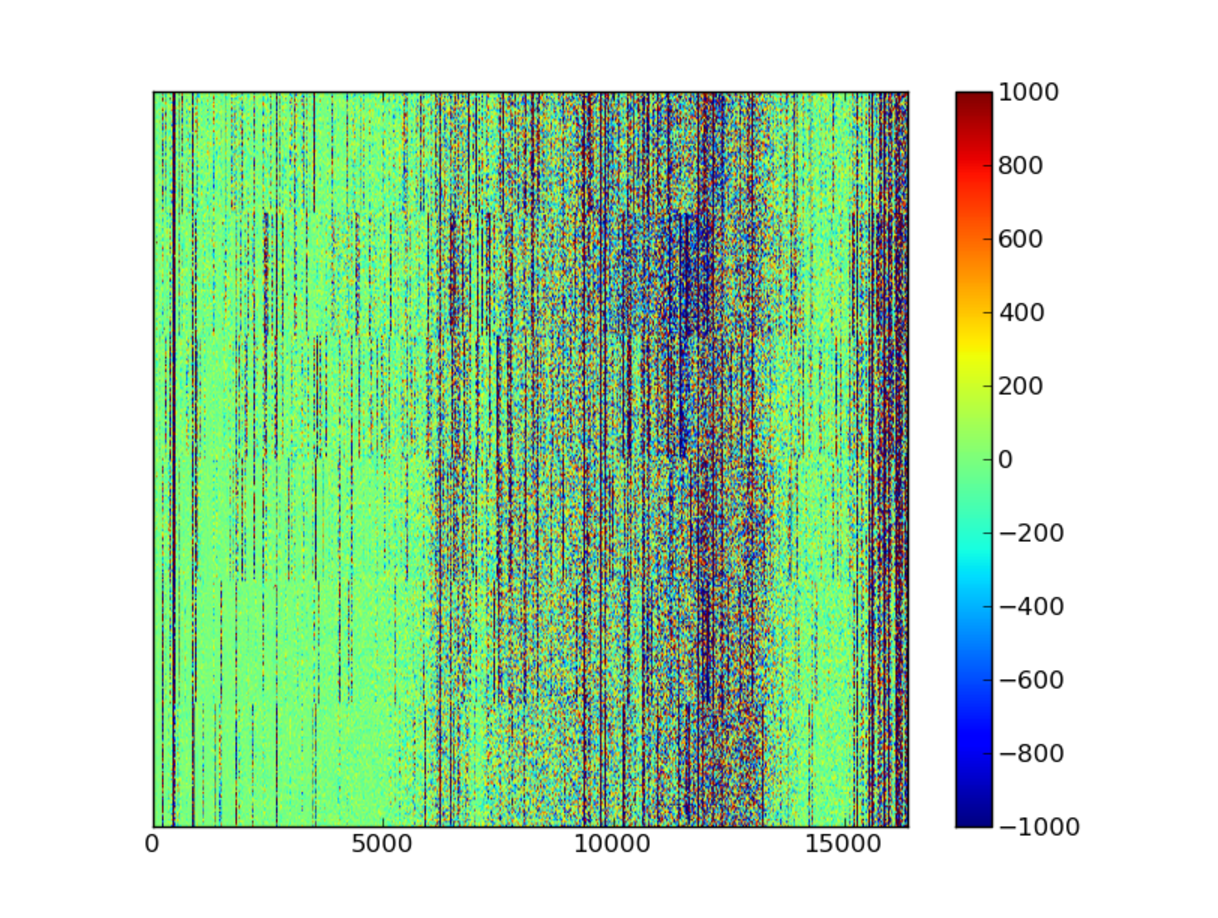
\includegraphics[width=1.3\linewidth]{1810fig1node9.pdf}
  \label{fig:sub1810node9}
\end{subfigure}%
\begin{subfigure}{0.5\textwidth}
  \centering
  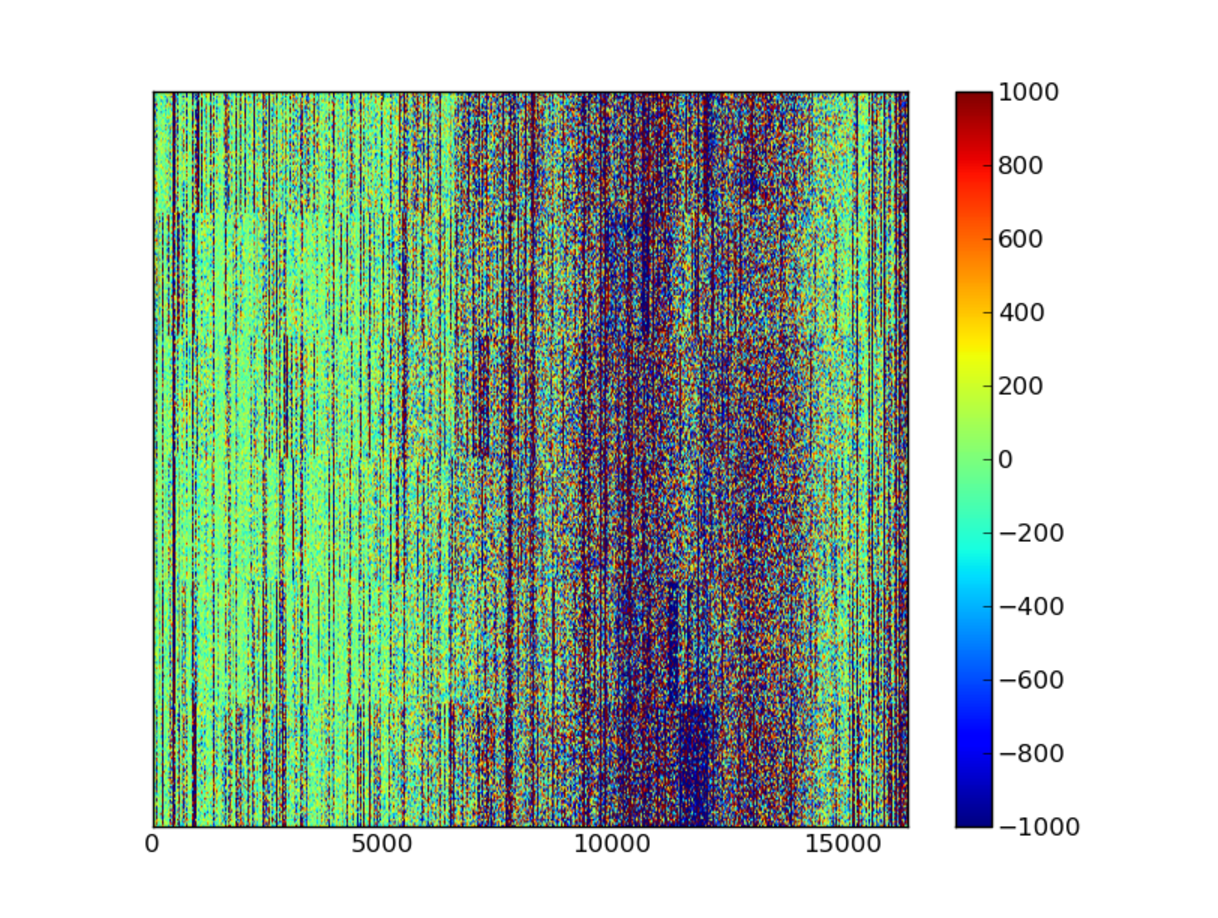
\includegraphics[width=1.3\linewidth]{1810fig2node7.pdf}
  \label{fig:sub1810node7}
\end{subfigure}
\caption{Plots of both polarizations of the millisecond pulsar J1810+1744 folded over an hour and a half with 16384 frequency channels and divided into 6 time bins along the y-axis. The x-axis is the number of the frequency bin, the colourbar the intensity of the signal. The left plot is the polarization recorded onto node9, the right is the polarization recorded onto node7. In neither is the pulsar visible. Data was taken on July 24 2013.}
\label{fig:folding1810}
\end{figure}



\bibliographystyle{plainnat}
\bibliography{cite}

\end{document}